\documentclass{beamer}
\usetheme{metropolis}           % Use metropolis theme
\usepackage{appendixnumberbeamer}
\usepackage{epigraph}
\usepackage{color}
\usepackage{amsopn}
\usepackage{tabto}

%%% Bibliography
\usepackage[backend=bibtex, style=authoryear]{biblatex}
\AtBeginBibliography{\tiny}
\bibliography{../src/bibliography.bib}

%\setbeamercolor{background canvas}{bg=white}
%\setbeamercolor{title}{fg=white}
%\setbeamercolor{subtitle}{fg=black}
%\setbeamercolor{author}{fg=black}
%\setbeamercolor{institute}{fg=white}

\newcommand{\todo}{\alert{TODO}}
\newcommand{\itemBullet}{\scriptsize$\blacksquare$}
\setbeamertemplate{itemize item}{\itemBullet}
\setbeamertemplate{itemize subitem}{\itemBullet}
\setbeamertemplate{itemize subsubitem}{\itemBullet}
\newcommand{\E}{\mathop{\mathbb{E}}}
\DeclareMathOperator*{\argmax}{arg\,max}
\newcommand{\epiParSpace}{\vskip 1.5ex}
\newcommand{\vect}[1]{\boldsymbol{#1}}
\newcommand{\I}{\mathcal{I}}

\title{Solving Endgames \\in~Large Imperfect-Information Games \\such as~Poker}
\date{September 13, 2016}
\author{Bc.~Karel Ha}
\institute{Department of~Applied Mathematics \\Charles University}

\begin{document}
  \maketitle

  % todo df: subgame / endgame
  % todo application in game playing

  \section{Perfect-Information Subgames}
  % todo Lomonosov chess
  % todo Go CGT
  % todo Go AlphaGo

  \section{Imperfect-Information Subgames}
  % todo df: (imperf-info) subgame
  % todo solving games: sequences, sequence-form LP
  % todo solving games: learning algos

  \section{Endgame Solving}
  {
    \setbeamercolor{background canvas}{bg=white}
    \begin{frame}{Endgame Solving: Gadget Game}
      \begin{figure}
        \centering
        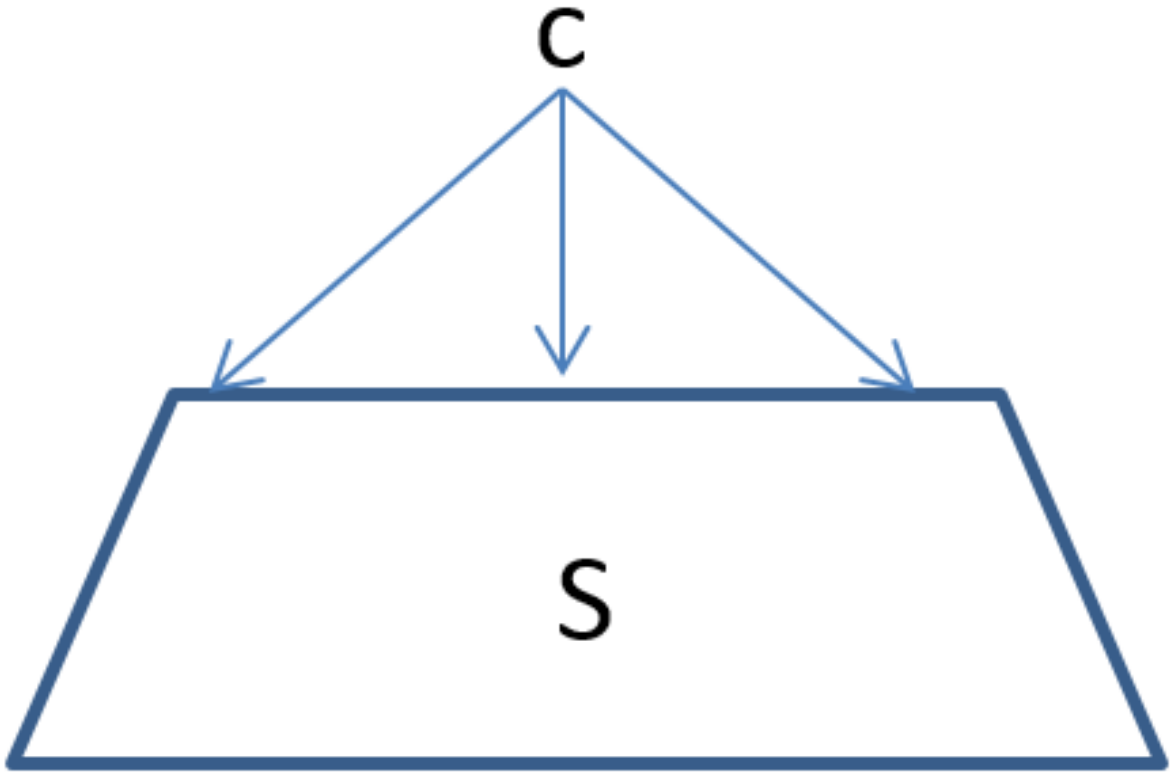
\includegraphics[width=.5\textwidth]{../img/endgame-solving-gadget.png}
      \end{figure}
    \end{frame}
  }

  \begin{frame}{Endgame Solving: Linear Program}
    \begin{equation*}
      \label{lp:endgame-solving}
      \begin{split}
        \max_{v, x}\  f^\top v & \\
        Ex &= e \\
        F^\top v - A^\top x &\le \vect{0} \\
        x &\ge \vect{0}
      \end{split}
    \end{equation*}
  \end{frame}

  \section{CFR-D Decomposition}
  {
    \setbeamercolor{background canvas}{bg=white}
    \begin{frame}{CFR-D Decomposition: Gadget Game}
      \begin{figure}[H]
        \centering
        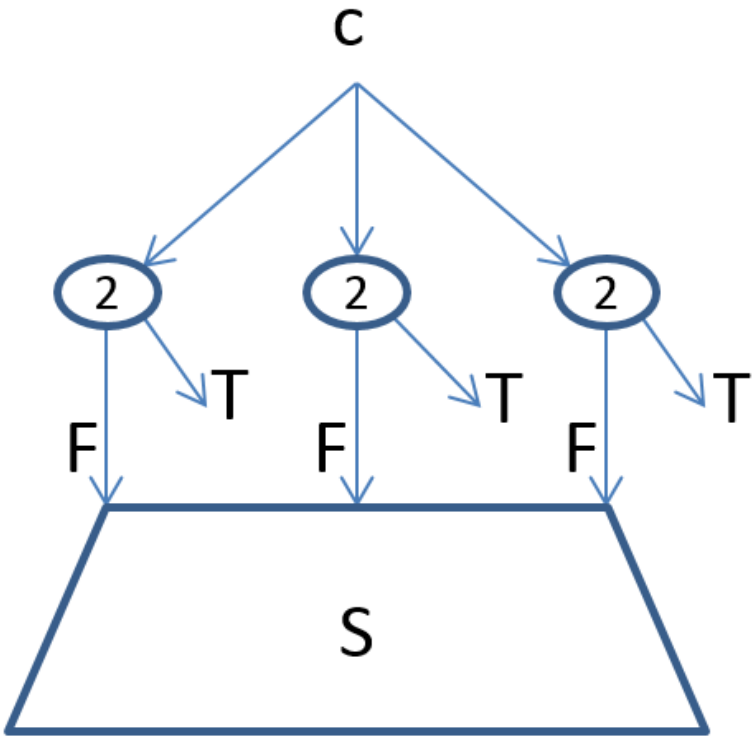
\includegraphics[width=.4\textwidth]{../img/re-solving-game-gadget.png}
      \end{figure}
      \pause

      \begin{itemize}[<+- | alert@+>]
        \item choice of~either to (F)ollow the action into the endgame, or to (T)erminate
        \item utility after the (T)erminal action set to the \emph{counterfactual best-response value}
      \end{itemize}
    \end{frame}
  }
  % todo LP

  \section{Subgame-Margin Maximization}
  % todo df: margin
  % todo thm: improvement-propto-margin
  % todo LP
  % todo gadget

  \section{Ideas for Future Work}

  \begin{frame}{Margins as a~Vector Linear Program}
    \begin{equation*}
      \label{vlp:max-margins}
      \begin{split}
        \max_{v, x}\ &\textcolor{red}{\vect{m}} \\
        v_I - \vect{m}_{\textcolor{red}{I}} &\ge CBV_2^{\sigma_1}(I), \quad I \in \I_2^{R(S)}\\ 
        Ex &= e \\
        F^\top v - A_2^\top x &\le \vect{0} \\
        x &\ge \vect{0}
      \end{split}
    \end{equation*}

    \pause
    \begin{itemize}[<+- | alert@+>]
      \item $\vect{m}_I := CBV_2^{\sigma_1} (I) - CBV_2^{\sigma_1'} (I)$ corresponds to one specific margin
      \item $\vect{m} := (m_I) _{I\in\I_2^{R(S)}}$ is a~vector of~all such margins
      \item multi-criteria optimization problem
      \item corresponding gadget games?
    \end{itemize}
  \end{frame}

  \begin{frame}[standout]
    \begin{center}
      Thank you!
    \end{center}
  \end{frame}

%%%%%%%%%%%%%%%%%%%%%%%%%%%%%%%%%%%%%%%%%%%%%%%%%%%%%%%%%%%%%%%%%%%%%%%%%%%%%%%%

  \begin{frame}[allowframebreaks]{References}
    \tiny
    \printbibliography[heading=none]
  \end{frame}

\end{document}
